%------------------------------------------
%       $Id: GMT_Tutorial.tex,v 1.78 2011-07-12 02:02:39 remko Exp $
%
%       The GMT Documentation Project
%	Copyright (c) 2000-2011.
%	P. Wessel, W. H. F. Smith, R. Scharroo, and J. Luis
%------------------------------------------
%
\documentclass{report}
\newcommand{\GMTTITLE}{A Map-making Tutorial}
\usepackage{ifpdf}
\usepackage{graphicx}
\usepackage{makeidx}
\usepackage{a4wide}
\usepackage{float}
\usepackage{GMT}
\usepackage{times}
\usepackage{color}
\usepackage{mathptmx}
\usepackage{verbatim}
\usepackage{tocbibind}
\usepackage{html}% Implies \usepackage{hyperref}

\input{GMT_version}

\newcommand{\GMTSITE}{gmt.soest.hawaii.edu}

\ifpdf
   % Here for creating PDF output with pdfLaTeX
   \pdfcompresslevel=9
   \DeclareGraphicsExtensions{.pdf}
   \hypersetup{%
      pdfauthor={Paul Wessel, Walter H. F. Smith},
      pdftitle={The Generic Mapping Tools Version \GMTDOCVERSION---\GMTTITLE},
      pdfsubject={GMT: Generic Mapping Tools},
      pdfkeywords={GMT, projections, mapping},
      pdfcreator={pdfLaTeX},
      bookmarksopen=true,
      bookmarksnumbered=true,
      hypertexnames=true,
      breaklinks=true,
      %pdfstartview={FitH},
      %linkbordercolor={1 1 0},
      %urlbordercolor={1 0 0},
   }%
   \newcommand{\GMT}{\textit{GMT}}
   \newcommand{\gmt}{\href{http://\GMTSITE}{\textbf{GMT}}}
   \newcommand{\GMTprogi}[1]{\htmladdnormallink{\textsfbf{#1}}{../html/#1.html}}
\else
   % Here for creating PS or HTML output with LaTeX
   \DeclareGraphicsExtensions{.eps}
   \newcommand{\GMT}{\htmladdnormallink{\includegraphics{fig/GMT_glyph10.eps}}{http://\GMTSITE}}
   \newcommand{\gmt}{\htmladdnormallink{GMT}{http://\GMTSITE}}
   \newcommand{\GMTprogi}[1]{\htmladdnormallink{\textsfbf{#1}}{../#1.html}}
\fi

\pagecolor{white}

% GMTfig will insert an eps file, add a label, and set a caption
\newcommand{\GMTfig}[3][tbp]{\begin{figure}[#1]\centering\includegraphics{scripts/#2}\caption{#3}\label{fig:#2}\end{figure}}
% Same for examples (scales by 50% by default)
\newcommand{\GMTexample}[3][scale=0.5]{\begin{figure}[hbtp]\centering\includegraphics[#1]{scripts/example_#2}\caption{#3}\label{fig:GMT_example_#2}\end{figure}}
\newcommand{\GMTanimation}[3][scale=0.5]{\begin{figure}[hbtp]\centering\includegraphics[#1]{scripts/anim_#2}\caption{#3}\label{fig:GMT_animation_#2}\end{figure}}

\newcommand{\PS}{\textit{PostScript}}
\newcommand{\UNIX}{\textit{UNIX}}
\newcommand{\id}[1]{#1\index{#1}}

\newcommand{\textsfbf}[1]{{\sffamily\bfseries #1\/}}
\newcommand{\textslbf}[1]{{\slshape\bfseries #1\/}}

\newcommand{\GMTprog}[1]{\GMTprogi{#1}\index{#1@\textsfbf{#1}}}

\newcommand{\script}[1]{%
   \begingroup
   \scriptsize\vspace{0.25\baselineskip}\noindent\hrulefill\vspace{-0.75\baselineskip}%
   \verbatiminput{scripts/#1.tex}%
   \vspace{-1.25\baselineskip}\noindent\hrulefill\vspace{0.25\baselineskip}%
   \endgroup
}

\newcommand{\GMTfunc}[1]{\texttt{#1}}
\newcommand{\filename}[1]{\underline{#1}}

\setcounter{topnumber}{2}
\renewcommand{\topfraction}{.8}
\setcounter{bottomnumber}{1}
\renewcommand{\bottomfraction}{.7}
\setcounter{totalnumber}{3}
\renewcommand{\textfraction}{.2}
\renewcommand{\floatpagefraction}{.7}

\sloppy

\newcommand{\DS}{$^{\circ}$}
\newcommand{\PM}{$\pm$}
\newcommand{\progname}[1]{\textslbf{#1}\index{#1@\textslbf{#1}}}
\newcommand{\Opt}[1]{\textbf{--#1}}

% Now overrule a few things for running LaTeX2HTML.
% Note that we need \gdef because they are inside an environment and would otherwise be local to
% that.
\begin{htmlonly}
   \gdef\GMT{\htmladdnormallink{\textbf{GMT}}{http://\GMTSITE}}
   \gdef\gmt{\GMT}
   \gdef\script#1{\htmlrule\verbatiminput{scripts/#1.tex}\htmlrule}
   \gdef\DS{�}
   \gdef\Opt#1{\textbf{-#1}}
   \gdef\PM{�}
   \gdef\progname#1{\textit{#1}\index{#1@\textit{#1}}}
\end{htmlonly}

% Restrict the indentation of lists
\setlength\leftmargin\parindent
\setlength\leftmargini\parindent
\setlength\leftmarginii\parindent
\setlength\leftmarginiii\parindent
\setlength\leftmarginiv\parindent
\setlength\leftmarginv\parindent
\setlength\leftmarginvi\parindent

\makeindex

%--------------------------------------------------------------------------
\begin{document}

\pagenumbering{roman}
%------------------------------------------
%       $Id: GMT_Cover.tex,v 1.28 2011-04-18 19:30:27 remko Exp $
%
%       The GMT Documentation Project
%	Copyright (c) 2000-2011.
%	P. Wessel, W. H. F. Smith, R. Scharroo, and J. Luis
%------------------------------------------
%

\thispagestyle{empty}

\begin{center}
\Huge
\textbf{The Generic Mapping Tools}\par 
\vspace{0.5\baselineskip}
\textbf{\GMTTITLE}\par 

\large
\vspace{0.5\baselineskip}
\textbf{Version \GMTDOCVERSION, \GMTDOCDATE}\par 
\vspace{0.25\baselineskip}

\vspace{2.0\baselineskip}

\huge
\textbf{P\aa l (Paul) Wessel}\par 
\vspace{0.5\baselineskip}

\Large
\textbf{SOEST, University of Hawai'i at M\={a}noa}\par 
\vspace{0.5\baselineskip}

\huge
\textbf{Walter H. F. Smith}\par 
\vspace{0.5\baselineskip}

\Large
\textbf{Laboratory for Satellite Altimetry, NOAA/NESDIS}\par 
\vspace{0.5\baselineskip}

\huge
\textbf{Remko Scharroo}\par 
\vspace{0.5\baselineskip}

\Large
\textbf{Altimetrics LLC, Cornish, New Hampshire}\par 
\vspace{0.5\baselineskip}

\huge
\textbf{Joaquim Luis}\par 
\vspace{0.5\baselineskip}

\Large
\textbf{Universidade do Algarve, Faro, Portugal}\par 
\vspace{0.5\baselineskip}



\includegraphics{GMT_coverlogo}
\end{center}

\addcontentsline{toc}{chapter}{Front page}
\clearpage

\thispagestyle{headings}
\tableofcontents 
%\addcontentsline{toc}{chapter}{Contents}

\chapter*{INTRODUCTION} 
\pagenumbering{arabic}
\thispagestyle{headings}
\addcontentsline{toc}{chapter}{INTRODUCTION}
\index{Purpose of tutorial}

The purpose of this tutorial is to introduce new users to \GMT,
outline the \GMT\ environment, and enable you to make several
forms of graphics without having to know too much about \UNIX\
and \UNIX\ tools.  We will not be able to cover all aspects of
\GMT\ nor will we necessarily cover the selected topics in
sufficient detail.  Nevertheless, it is hoped that the exposure
will prompt the users to improve their \GMT\ and \UNIX\ skills
after completion of this short tutorial.

\section*{\gmt\ overview: History, philosophy, and usage}
\addcontentsline{toc}{section}{\gmt\ overview: History, philosophy, and usage}

\subsection*{Historical highlights}
\addcontentsline{toc}{subsection}{Historical highlights}
\index{GMT@\GMT!history}

The \GMT\ system was initiated in late 1987 at Lamont-Doherty
Earth Observatory, Columbia University by graduate students Paul
Wessel and Walter H. F. Smith.  Version 1 was officially introduced
to Lamont scientists in July 1988.  \GMT\ 1 migrated by word of mouth
(and tape) to other institutions in the United States, UK, Japan, and
France and attracted a small following.  Paul took a Post-doctoral
position at SOEST in December 1989 and continued the \GMT\ development.
Version 2.0 was released with an article in EOS, October 1991, and
quickly spread worldwide.  We obtained NSF-funding for \GMT\
version 3.0 in 1993 which was released with another article in EOS
on August 15, 1995.  Significantly improved versions (3.1-3.3,
3.3.1--6), 3.4, 3.4.1--5, and 4.0--4.5.0 were released between November 1998 and
July 2009, culminating in the \GMTDOCDATE\ introduction of \GMTDOCVERSION.
\GMT\ now is used by $\sim$15,000 users worldwide in a broad range of disciplines.

\subsection*{Philosophy}
\addcontentsline{toc}{subsection}{Philosophy}
\index{GMT@\GMT!philosophy}

\GMT\ follows the \UNIX\ philosophy in which complex tasks are broken
down into smaller and more manageable components.  Individual \GMT\
modules are small, easy to maintain, and can be used as any other
\UNIX\ tool.  \GMT\ is written in the ANSI C programming language
(very portable), is POSIX compliant, and is independent of
hardware constraints (e.g., memory).  \GMT\ was deliberately written
for command-line usage, not a windows environment, in order to
maximize flexibility.  We standardized early on to use \PS\ output
instead of other graphics formats.  Apart from the built-in support for
coastlines, \GMT\ completely decouples data retrieval from the main
\GMT\ programs.  \GMT\ uses architecture-independent file formats.

\subsection*{Why is \gmt\ so popular?}
\addcontentsline{toc}{subsection}{Why is \gmt\ so popular?}
\index{GMT@\GMT!popularity}

The price is right!  Also, \GMT\ offers unlimited flexibility since
it can be called from the command line, inside scripts, and from user
programs.  \GMT\ has attracted many users because of its high quality
\PS\ output.  \GMT\ easily installs on almost any computer.

\subsection*{\gmt\ installation considerations}
\addcontentsline{toc}{subsection}{\gmt\ installation considerations}
\index{GMT@\GMT!installation}

\GMT\ has been installed on machines ranging from super-computers
to lap-top PCs.  \GMT\ only contains some 100,000 lines of code and
has modest space/memory requirements.  Minimum requirements are
\index{GMT@\GMT!requirements}

\begin{itemize}

\item The netCDF library 3.4 or higher (free from www.unidata.edu).
\item A C Compiler (free from www.gnu.org).
\item About 100 Mb disk space (70 Mb additional for full- and
high-resolution coast-lines).
\item About 32 Mb memory.

\end{itemize}

In addition, we recommend access to a \PS\ printer or equivalent
(e.g., \progname{ghostscript}), \PS\ previewer (e.g., \progname{ghostview}),
any flavor of the \UNIX\ operating system, and more disk space and memory.

\chapter{SESSION ONE} 
\thispagestyle{headings}

\section{Tutorial setup}
\begin{enumerate}

\item We assume that \GMT\ has been properly and fully
installed and that the \GMT\ executables are in your executable path
described in the \GMT\ \filename{README} file.

\item All \GMT\ man pages, documentation, and example scripts
are available from the \GMT\ documentation web page.  It is
assumed these pages have been installed locally at your site;
if not they are always available from the main
\htmladdnormallinkfoot{GMT home page}{http://\GMTSITE}.

\item We recommend you create a sub-directory called \filename{tutorial},
cd into that directory, and copy all the tutorial files directly
there. Depending on your installation the tutorial files are likely in \filename{/usr/share/doc/gmt/tutorial}.

\item As we discuss \GMT\ principles it may be a good idea to
consult the \GMT\ Technical Reference and Cookbook for more
detailed explanations.

\item The tutorial uses the supplemental \GMT\ program
\GMTprog{grdraster} to extract subsets of global gridded data
sets.  For your convenience we also supply the subsets in the
event you do not wish to install \GMTprog{grdraster} and the
public data sets it can read.  Thus, run the \GMTprog{grdraster}
commands if you have made the installation or ignore them if
you have not.

\item For all but the simplest \GMT\ jobs it is recommended that
you place all the \GMT\ (and \UNIX) commands in a shell script
file and make it executable.  To ensure that \UNIX\ recognizes
your script as a shell script it is a good habit always to start
the script with the line \#!/bin/sh or \#!/bin/csh, depending on the shell you prefer to use.
All the examples in this tutorial assumes you are running the bourne shell, \progname{sh}; if you are using
something different then you are on your own.

\item Making a script executable is accomplished using the \texttt{chmod}
command, e.g., the script \filename{figure\_1.sh} is made executable
with ``\texttt{chmod +x figure\_1.sh}''.

\item To view a \PS\ file (e.g., \filename{map.ps}) on a UNIX workstation
we use \progname{ghostview} \filename{map.ps}.  On some systems there
will be similar commands, like \filename{imagetool} and \filename{pageview}
on Sun workstations.  In this text we will refer to
\progname{ghostview}; please substitute the relevant \PS\ previewer
on your system.

\item Please cd into the directory \filename{tutorial}.  We are
now ready to start.

\end{enumerate}

\section{The \gmt\ environment: What happens when you run \gmt ?}
\index{GMT@\GMT!environment}
\index{Run-time environment}

To get a good grasp on \GMT\ one must understand what is going on ``under
the hood''.  Figure~\ref{fig:GMT_Environment} illustrates the relationships
you need to be aware of at run-time.

\begin{figure}[h]
   \centering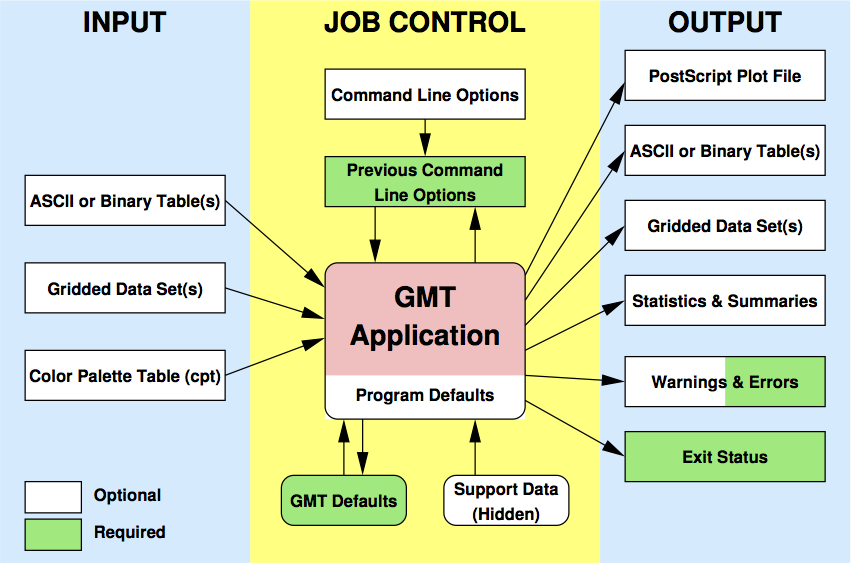
\includegraphics[width=0.8\textwidth]{GMT_Environment}
   \caption{The \gmt\ run-time environment.}
   \label{fig:GMT_Environment}
\end{figure}

\subsection{Input data}
A \GMT\ program may or may not take input files.  Three different
types of input are recognized (more details can be found in Appendix
B in the Technical Reference):
\index{GMT@\GMT!input}
\index{Input files}

\begin{enumerate}

\item Data tables.
These are ``spreadsheet'' tables with a fixed number of columns and
unlimited number of rows.  We distinguish between two groups:

\begin{itemize}

\item ASCII (Preferred unless files are huge)

\begin{itemize}

\item Single segment [Default]

\item Multi-segment with internal header records (\Opt{M})
\end{itemize}

\item Binary (to speed up input/output)

\begin{itemize}

\item Single segment [Default]

\item Multi-segment (segment headers are all NaN fields) (\Opt{M})
\end{itemize}

\end{itemize}

\item Gridded dated sets.
These are data matrices (evenly spaced in two coordinates) that come
in two flavors:

\begin{itemize}

\item Grid-line registration

\item Pixel registration

\end{itemize}

You may choose among several file formats (even define your own format),
but the \GMT\ default is the architecture-indenpendent netCDF format.

\item Color palette table (For imaging, color plots, and contour maps).
We will discuss these later.

\end{enumerate}

\subsection{Job Control}

\GMT\ programs may get operational parameters from several places:

\begin{enumerate}

\item Supplied command line options/switches or program defaults.

\item Short-hand notation to select previously used option arguments
(stored in \filename{.gmtcommands}).
\index{gmt.conf@\filename{gmt.conf}}

\item Implicitly using \GMT\ defaults for a variety of parameters
(stored in \filename{gmt.conf}).

\item May use hidden support data like coastlines or \PS\ patterns.

\end{enumerate}

\subsection{Output data}
There are 6 general categories of output produced by \GMT:

\begin{enumerate}

\item \PS\ plot commands.

\item Data Table(s).

\item Gridded data set(s).

\item Statistics \& Summaries.

\item Warnings and Errors, written to \emph{stderr}.

\item Exit status (0 means success, otherwise failure).

\end{enumerate}

Note: \GMT\ automatically creates and updates a history of past
\GMT\ command options for the common switches.  This history
file is called \filename{.gmtcommands} and one will be created in
every directory from which \GMT\ programs are executed.  Many
initial problems with \GMT\ usage result from not fully appreciating
the relationships shown in Figure~\ref{fig:GMT_Environment}.

\section{The UNIX Environment: Entry Level Knowledge}

\subsection{Redirection}
\index{UNIX@\UNIX!redirection}
\index{Redirection}

Most \GMT\ programs read their input from the terminal (called
\emph{stdin}) or from files, and write their output to the
terminal (called \emph{stdout}).  To use files instead one can
use \UNIX\ redirection:

{\small\begin{verbatim}
GMTprogram input-file > output-file
GMTprogram < input-file > output-file
GMTprogram input-file >> output-file       # Append to existing file
\end{verbatim}
}

\noindent
In this example, and in all those to follow, it is assumed that you do not have the shell
variable \textbf{noclobber} set. If you do, it prevents accidental overwriting of existing files.
That may be a noble cause, but it is extremely annoying. So please, \textbf{unset noclobber}.

\subsection{Piping ($|$)}
\index{UNIX@\UNIX!piping}
\index{Piping}

Sometimes we want to use the output from one program as input
to another program.  This is achieved with \UNIX\ pipes:

{\small\begin{verbatim}
Someprogram | GMTprogram1 | GMTprogram2 > Output-file (or | lp) 
\end{verbatim}
}

\subsection{Standard error (\emph{stderr})}
\index{UNIX@\UNIX!stderr}
\index{Standard error}

Most \UNIX\ and \GMT\ programs will on occasion write error messages.
These are typically written to a separate data stream called
\emph{stderr} and can be redirected separately from the standard
output (which goes to \emph{stdout}).  To send the error messages to the same location
as standard output we use

{\small\begin{verbatim}
UNIXprogram > errors.log 2>&1
\end{verbatim}
}

When we want to save both program output and error messages to
separate files we use the following syntax:

{\small\begin{verbatim}
GMTprogram > output.d 2> errors.log
\end{verbatim}
}

\subsection{File name expansion or ``wild cards''}
\index{Wild cards@``Wild cards''}
\index{UNIX@\UNIX!``wild cards''}

\UNIX\ provides several ways to select groups of files based
on name patterns (Table~\ref{tbl:wildcard}):

\begin{table}[h]
\small
\centering
\begin{tabular}{|l|l|} \hline
\multicolumn{1}{|c|}{\emph{Code}} & \multicolumn{1}{c|}{\emph{Meaning}} \\ \hline
*       &       Matches anything \\ \hline
?       &       Matches any single character \\ \hline
[\emph{list}]   &       Matches characters in the list \\ \hline
[\emph{range}]  &       Matches characters in the given range \\ \hline
\end{tabular}
\caption{\UNIX\ wildcards.} \label{tbl:wildcard}
\end{table}
 
\noindent
You can save much time by getting into the habit of selecting
``good'' filenames that make it easy to select subsets of all
files using the \UNIX\ wild card notation.

\subsubsection{Examples}
\index{Examples|(}

\begin{itemize}
\item GMTprogram data\_*.d operates on all files starting with
``data\_'' and ending in ``.d''.

\item GMTprogram line\_?.d works on all files starting with
``line\_'' followed by any single character and ending in ``.d''.

\item GMTprogram section\_1[0-9]0.part\_[12] only processes data
from sections 100 through 190, only using every 10th profile, and
gets both part 1 and 2.

\end{itemize} 
\index{Examples|)}

\section{Laboratory Exercises}

We will begin our adventure by making some simple plot axes and
coastline basemaps.  We will do this in order to introduce the all-%
important \Opt{B}, \Opt{J}, and \Opt{R} switches and to familiarize
ourselves with a few selected \GMT\ projections.  The \GMT\ programs
we will utilize are \GMTprog{psbasemap} and \GMTprog{pscoast}.  Please
consult their manual pages on the \GMT\ web site for reference.

\subsection{Linear projection}
\index{Linear projection \Opt{JX}}
\index{Projection!linear}

We start by making the basemap frame for a linear \emph{x-y} plot.
We want it to go from 10 to 70 in \emph{x}, annotating every 10, and
from -3 to 8 in \emph{y}, annotating every 1.  The final plot should be
4 by 3 inches in size.  Here's how we do it:

{\small\begin{verbatim}
psbasemap -R10/70/-3/8 -JX4i/3i -B10/1:."My first plot": -P > plot.ps
\end{verbatim}
}

\noindent
You can view the result with \progname{ghostview} \filename{plot.ps}.

\subsubsection{Exercises}
\index{Exercises|(}

\begin{enumerate}

\item Try change the \Opt{JX} values.

\item Try change the \Opt{B} values.

\item Omit the \Opt{P}.

\end{enumerate}
\index{Exercises|)}

\subsection{Logarithmic projection}
\index{Logarithmic projection}
\index{Projection!logarithmic}

We next will show how to do a basemap for a log--log plot.  We will
assume that the raw \emph{x} data range from 3 to 9613 and \emph{y}
ranges from $3.2 \cdot 10^{20}$ to $6.8 \cdot 10^{24}$.  One possibility is

{\small\begin{verbatim} 
psbasemap -R1/10000/1e20/1e25 -JX9il/6il \
   -B2:"Wavelength (m)":/a1pf3:"Power (W)":WS > plot.ps 
\end{verbatim}
}

\noindent
(The backslash $\backslash$ makes \UNIX\ ignore the carriage return that follows and treat the two lines as one long command).

\subsubsection{Exercises}
\index{Exercises|(}

\begin{enumerate}

\item Do not append \textbf{l} to the axes lengths.

\item Leave the \textbf{p} modifier out of the \Opt{B} string.

\item Add \textbf{g}3 to each side of the slash in \Opt{B}.

\end{enumerate}
\index{Exercises|)}

\subsection{Mercator projection}
\index{Mercator projection \Opt{JM}}
\index{Projection!Mercator}

Despite the problems of extreme horizontal exaggeration at high
latitudes, the conformal Mercator projection (\Opt{JM}) remains
the stalwart of location maps used by scientists.  It is one
of several cylindrical projections offered by \GMT; here we
will only have time to focus on one such projection.  The
complete syntax is simply \\

\Opt{JM}\emph{width} \\

To make coastline maps we use \GMTprog{pscoast} which automatically will
access the \GMT\ coastline data base derived from the GSHHS
database\footnote{See \emph{Wessel and Smith} [1996].}.  In addition
to the common switches we may need to use some of several \GMTprog{pscoast}
-specific options (see Table~\ref{tbl:pscoast}).

\begin{table}[h]
\small
\centering
\begin{tabular}{|l|l|} \hline
\multicolumn{1}{|c|}{\emph{Option}} & \multicolumn{1}{c|}{\emph{Purpose}} \\ \hline 
\Opt{A} & Exclude small features or those of high hierarchical levels (see Appendix K)\\ \hline
\Opt{D} & Select data resolution (\textbf{f}ull, \textbf{h}igh, \textbf{i}ntermediate, \textbf{l}ow, or \textbf{c}rude) \\ \hline
\Opt{G} & Set color of dry areas (default does not paint) \\ \hline
\Opt{I} & Draw rivers (chose features from one or more hierarchical categories) \\ \hline
\Opt{L} & Plot map scale (length scale can be km, miles, or nautical miles) \\ \hline
\Opt{N} & Draw political borders (including US state borders) \\ \hline
\Opt{S} & Set color for wet areas (default does not paint) \\ \hline
\Opt{W} & Draw coastlines and set pen thickness \\ \hline
\end{tabular}
\caption{Main options when making coastline plots or overlays.} \label{tbl:pscoast}
\end{table}

One of \Opt{W}, \Opt{G}, \Opt{S} must be selected.  Our first coastline
example is from Latin America:

{\small\begin{verbatim}
pscoast -R-90/-70/0/20 -JM6i -P -B5g5 -Gchocolate > map.ps 
\end{verbatim}
}

\subsubsection{Exercises}
\index{Exercises|(}

\begin{enumerate}

\item Add the \Opt{V} option.

\item Try \Opt{R}270/290/0/20 instead.  What happens to the annotations?

\item Edit your \filename{gmt.conf} file, change \textbf{FORMAT\_GEO\_MAP}
to another setting (see the \GMTprog{gmt.conf} man page), and plot again.

\item Pick another region and change land color.

\item Pick a region that includes the north or south poles.

%\item Try \Opt{W}0.25\textbf{p} instead of (or in addition to) \Opt{G}.

\item Try \Opt[0.25{\textbf{p}}]{W} instead of (or in addition to) \Opt{G}.

\end{enumerate}
\index{Exercises|)}

\subsection{Albers projection}
\index{Albers projection \Opt{JB}}
\index{Projection!Albers}

The Albers projection (\Opt{JB}) is an equal-area conical projection;
its conformal cousin is the Lambert conic projection (\Opt{JL}).
Their usages are almost identical so we will only use the Albers here.
The general syntax is \\

%\Opt{JB}$lon_0/lat_0/lat_1/lat_2/width$ \\
\Opt[$lon_0/lat_0/lat_1/lat_2/width$]{JB} \\

\noindent
where ($lon_0, lat_0$) is the map (projection) center and $lat_1, lat_2$
are the two standard parallels where the cone intersects the Earth's surface.
We try the following command:

{\small\begin{verbatim}
pscoast -R-130/-70/24/52 -JB-100/35/33/45/6i -B10g5:."Conic Projection": \
   -N1/thickest -N2/thinnest -A500 -Ggray -Wthinnest -P > map.ps
\end{verbatim}
}

\subsubsection{Exercises}
\index{Exercises|(}

\begin{enumerate}

\item Change the parameter \textbf{MAP\_GRID\_CROSS\_SIZE\_PRIMARY} to make grid crosses instead of gridlines.

\item Change \Opt{R} to a rectangular box specification instead of
minimum and maximum values.

\end{enumerate}
\index{Exercises|)}

\subsection{Orthographic projection}
\index{Orthographic projection \Opt{JG}}
\index{Projection!orthographic}

The azimuthal orthographic projection (\Opt{JG}) is one of several
projections with similar syntax and behavior; the one we have
chosen mimics viewing the Earth from space at an infinite distance;
it is neither conformal nor equal-area.
The syntax for this projection is \\

\Opt{JG}$lon_0/lat_0/width$ \\

\noindent
where ($lon_0, lat_0$) is the center of the map (projection).
As an example we will try

{\small\begin{verbatim}
pscoast -R0/360/-90/90 -JG280/30/6i -Bg30/g15 -Dc -A5000 -Gwhite \
    -SDarkTurquoise -P > map.ps
\end{verbatim}
}

\subsubsection{Exercises}
\index{Exercises|(}

\begin{enumerate}

\item Use the rectangular option in \Opt{R} to make a rectangular map
showing the US only.

\end{enumerate}
\index{Exercises|)}

\subsection{Eckert IV and VI projection}
\index{Eckert IV and VI projection \Opt{JK}}
\index{Projection!Eckert IV and VI}

We conclude the survey of map projections with the Eckert IV and VI projections
(\Opt{JK}), two of several projections used for global thematic maps; They
are both equal-area projections whose syntax is \\

%\Opt{JK}[\textbf{f$|$s}]$lon_0/width$ \\
\Opt[{$[${\textbf{f\textbar s}}$]lon_0/width$}]{JK} \\

\noindent
where \textbf{f} gives Eckert IV (4) and \textbf{s} (Default) gives Eckert VI (6).
The $lon_0$ is the central meridian (which takes precedence over
the mid-value implied by the \Opt{R} setting).  A simple Eckert VI world map
is thus generated by

{\small\begin{verbatim}
pscoast -R0/360/-90/90 -JKs180/9i -B60g30/30g15 -Dc -A5000 \
    -Gchocolate -SDarkTurquoise -Wthinnest > map.ps
\end{verbatim}
}

\subsubsection{Exercises}
\index{Exercises|(}

\begin{enumerate}

\item Center the map on Greenwich.

\item Add a map scale with \Opt{L}.

\end{enumerate}
\index{Exercises|)}

\chapter{SESSION TWO} 
\thispagestyle{headings}

\section{General Information}

There are 18 \GMT\ programs that directly create (or add overlays to)
plots (Table~\ref{tbl:plotprogs}); the remaining 45 are mostly concerned with data
processing.  This session will focus on the task of plotting
lines, symbols, and text on maps.  We will build on the skills
we acquired while familiarizing ourselves with the various
\GMT\ map projections as well as how to select a data domain
and boundary annotations.

\begin{table}[h]
\small
\centering
\begin{tabular}{|l|l|} \hline
\multicolumn{1}{|c|}{\emph{Program}} & \multicolumn{1}{c|}{\emph{Purpose}} \\ \hline 
\multicolumn{2}{|c|}{\emph{BASEMAPS}} \\ \hline
\GMTprog{psbasemap} & Create an empty basemap frame with optional scale \\ \hline
\GMTprog{pscoast} & Plot coastlines, filled continents, rivers, and political borders \\ \hline
\GMTprog{pslegend} & Create legend overlay \\ \hline
\multicolumn{2}{|c|}{\emph{POINTS AND LINES}} \\ \hline
\GMTprog{pswiggle} & Draw spatial time-series along their $(x,y)$-tracks \\ \hline
\GMTprog{psxy} & Plot symbols, polygons, and lines in 2-D \\ \hline
\GMTprog{psxyz} & Plot symbols, polygons, and lines in 3-D \\ \hline
\multicolumn{2}{|c|}{\emph{HISTOGRAMS}} \\ \hline
\GMTprog{pshistogram} & Plot a rectangular histogram \\ \hline
\GMTprog{psrose} & Plot a polar histogram(sector/rose diagram) \\ \hline
\multicolumn{2}{|c|}{\emph{CONTOURS}} \\ \hline
\GMTprog{grdcontour} & Contouring of 2-D gridded data sets \\ \hline
\GMTprog{pscontour} & Direct contouring or imaging of $xyz$ data by optimal triangulation \\ \hline
\multicolumn{2}{|c|}{\emph{SURFACES}} \\ \hline
\GMTprog{grdimage} & Produce color images from 2-D gridded data \\ \hline
\GMTprog{grdvector} & Plot vector fields from 2-D gridded data \\ \hline
\GMTprog{grdview} & 3-D perspective imaging of 2-D gridded data \\ \hline
\multicolumn{2}{|c|}{\emph{UTILITIES}} \\ \hline
\GMTprog{psclip} & Use polygon files to initiate custom clipping paths  \\ \hline
\GMTprog{psimage} & Plot Sun raster files \\ \hline
\GMTprog{psmask} & Create clipping paths or generate overlay to mask  \\ \hline
\GMTprog{psscale} & Plot gray scale or color scale bar \\ \hline
\GMTprog{pstext} & Plot text strings on maps \\ \hline
\end{tabular}
\caption{List of all 1-D and 2-D plotting programs in \gmt.}
\label{tbl:plotprogs}
\end{table}

Plotting lines and symbols, \GMTprog{psxy} is one of the most frequently
used programs in \GMT.  In addition to the common command line switches
it has numerous specific options, and expects different file formats
depending on what action has been selected.  These circumstances make
\GMTprog{psxy} harder to master than most \GMT\ tools.  Table~\ref{tbl:psxy}
shows a complete list of the options.

\begin{table}[h]
\small
\centering
\begin{tabular}{|l|l|} \hline
\multicolumn{1}{|c|}{\emph{Option}} & \multicolumn{1}{c|}{\emph{Purpose}} \\ \hline 
\Opt{A} & Suppress line interpolation along great circles \\ \hline
\Opt{C}\emph{CPT} & Let symbol color be determined from $z$-values and the \emph{CPT} file \\ \hline
\Opt{E}[\textbf{x}$|$\textbf{X}][\textbf{y}$|$\textbf{Y}][\emph{cap}][/\emph{pen}] & Draw selected error bars with specified attributes \\ \hline
\Opt{G}\emph{fill} & Set color for symbol or fill for polygons \\ \hline
\Opt{L} & Explicitly close polygons \\ \hline
\Opt{N} & Do Not clip symbols at map borders \\ \hline
\Opt{S[symbol]}[\emph{size}] & Select one of several symbols (See Table~\ref{tbl:psxysymbols}) \\ \hline
\Opt{W}\emph{pen} & Set \emph{pen} for line or symbol outline \\ \hline
\end{tabular}
\caption{Optional switches in the \protect\GMTprog{psxy} program.}
\label{tbl:psxy}
\end{table}

The symbols can either be transparent (using \Opt{W} only, not \Opt{G})
or solid (\Opt{G}, with optional outline using \Opt{W}).  The \Opt{S}
option takes the code for the desired symbol and optional size information.
If no symbol is given it is expected to be given in the last column of each record in the input
file.  The \emph{size} is optional since individual sizes for
symbols may also be provided by the input data.  The main symbols available to
us are shown in Table~\ref{tbl:psxysymbols}.

\begin{table}[h]
\index{Symbols, plot}
\index{Plot!symbols}
\small
\centering
\begin{tabular}{|l|l|} \hline
\multicolumn{1}{|c|}{\emph{Option}} & \multicolumn{1}{c|}{\emph{Symbol}} \\ \hline 
\Opt{S-}\emph{size} & horizontal dash; \emph{size} is length of dash \\ \hline
\Opt{Sa}\emph{size} & st\textbf{a}r; \emph{size} is radius of circumscribing circle \\ \hline
\Opt{Sb}\emph{size}[/\emph{base}][\textbf{u}] & \textbf{b}ar; \emph{size} is bar width, append \textbf{u} if \emph{size} is in
\emph{x}-units \\
 & Bar extends from \emph{base} [0] to the \emph{y}-value \\ \hline
\Opt{Sc}\emph{size} & \textbf{c}ircle; \emph{size} is the diameter \\ \hline
\Opt{Sd}\emph{size} & \textbf{d}iamond; \emph{size} is its side \\ \hline
\Opt{Se} & \textbf{e}llipse; \emph{direction} (CCW from horizontal), \emph{major}, and \emph{minor} axes in inches \\
 & are read from the input file \\ \hline
\Opt{SE} & \textbf{e}llipse; \emph{azimuth} (CW from vertical), \emph{major}, and \emph{minor} axes in kilometers \\
 & are read from the input file\\ \hline
\Opt{Sg}\emph{size} & octa\textbf{g}on; \emph{size} is its side \\ \hline
\Opt{Sh}\emph{size} & \textbf{h}exagon; \emph{size} is its side \\ \hline
\Opt{Si}\emph{size} & \textbf{i}nverted triangle; \emph{size} is its side \\ \hline
\Opt{Sk}\emph{symbol}/\emph{size} & \textbf{k}ustom symbol; \emph{size} is its side \\ \hline
\Opt{Sl}\emph{size}/\emph{string}[\%\emph{font}] & \textbf{l}etter; \emph{size} is fontsize.  Append a letter or text string, and optionally a font \\ \hline
\Opt{Sn}\emph{size} & pe\textbf{n}tagon; \emph{size} is its side \\ \hline
\Opt{Sp} & \textbf{p}oint; no size needed (1 pixel at current resolution is used) \\ \hline
\Opt{Sr}\emph{size} & \textbf{r}ect, \emph{width} and \emph{height} are read from input file \\ \hline
\Opt{Ss}\emph{size} & \textbf{s}quare, \emph{size} is its side \\ \hline
\Opt{St}\emph{size} & \textbf{t}riangle; \emph{size} is its side \\ \hline
\Opt{Sv}[\emph{thick}/\emph{length}/\emph{width}][\textbf{n}\emph{norm}] & \textbf{v}ector; \emph{direction} (CCW from
horizontal) and \emph{length} are read from input data \\
 & Optionally, append the thickness of the vector and the width and length of the \\
 & arrow-head.  If the \textbf{n}\emph{norm} is appended, all vectors whose lengths are less than \\
 & \emph{norm} will have their attributes scaled by length/\emph{norm} \\ \hline
\Opt{SV}[\emph{thick}/\emph{length}/\emph{width}][\textbf{n}\emph{norm}] & \textbf{v}ector, except \emph{azimuth} (degrees east
of north) is expected instead of \emph{direction} \\
 & The angle on the map is calculated based on the chosen map projection \\ \hline
\Opt{Sw}[\emph{size} & pie \textbf{w}edge; \emph{start} and \emph{stop} directions (CCW from horizontal) are read from \\
 & input data \\ \hline
\Opt{Sx}\emph{size} & cross; \emph{size} is length of crossing lines \\ \hline
\Opt{Sy}\emph{size} & vertical dash; \emph{size} is length of dash \\ \hline
\end{tabular}
\caption{The symbol option in \protect\GMTprog{psxy}.  Lower case symbols (\textbf{a, c, d, g, h, i, n, s, t, x})
will fit inside a circle of given diameter.  Upper case symbols (\textbf{A, C, D, G, H, I, N, S, T, X}) will have area equal to that of a circle of given diameter.}
\label{tbl:psxysymbols}
\end{table} 

Because some symbols require more input data than others, and because the
size of symbols as well as their color can be determined from the input data,
the format of data can be confusing.  The general format for the input data
is (optional items are in brackets []): \\
\index{psxy@\GMTprog{psxy} input format}

$x\mbox{  } y$ [ $z$ ] [ $size$ ] [ $\sigma_x$ ] [ $\sigma_y$ ] [ $symbol$ ] \\

Thus, the only required input columns are the first two which must contain the
longitude and latitude (or \emph{x} and \emph{y}).  The remaining items
apply when one (or more) of the following conditions are met:

\begin{enumerate}

\item If you want the color of each symbol to be determined individually,
supply a CPT file with the \Opt{C} option and let the 3rd data column
contain the \emph{z}-values to be used with the CPT file.

\item If you want the size of each symbol to be determined individually,
append the size in a separate column.

\item To draw error bars, use the \Opt{E} option and give one or two
additional data columns with the \PM dx and \PM dy values; the form of
\Opt{E} determines if one (\Opt{Ex} or \Opt{Ey}) or two (\Opt{Exy})
columns are needed.  If upper case flags \textbf{X} or \textbf{Y} are given then
we will instead draw a ``box-and-whisker'' symbol and the $\sigma_x$ (or
$\sigma_y$) must represent 4 columns containing the minimum, the 25 and 75\%
quartiles, and the maximum value.  The given $x$ (or $y$) coordinate is taken as the 50\%
quartile (median).
\index{Error bars}

\item If you draw vectors with \Opt{Sv} (or \Opt{SV}) then \emph{size} is
actually two columns containing the \emph{direction} (or \emph{azimuth})
and \emph{length} of each vector.
\index{Vectors}

\item If you draw ellipses (\Opt{Se}) then \emph{size} is actually three
columns containing the \emph{direction} and the \emph{major} and \emph{minor}
axes in plot units (with \Opt{SE} we expect \emph{azimuth} instead and axes
lengths in km).
\index{Ellipses}

\end{enumerate}

Before we try some examples we need to review two key switches; they
specify pen attributes and symbol or polygon fill.  Please consult
Chapter 4 in the \GMT\ Technical Reference and Cookbook before experimenting
with the examples below.

\subsection{Examples}
\index{Examples|(}

We will start off using the file \filename{data} in your directory.
Using the \GMT\ utility \GMTprog{minmax} we find the extent of the
data region:

{\small\begin{verbatim}
minmax data
\end{verbatim}
}

\noindent
which returns

{\small\begin{verbatim}
data: N = 7   <1/5>   <1/5>
\end{verbatim}
}

\noindent
telling us that the file \filename{data} has 7 records and gives the
minimum and maximum values for the first two columns.  Given our
knowledge of how to set up linear projections with \Opt{R} and \Opt{JX},
try the following:

\begin{enumerate}

\item Plot the data as transparent circles of size 0.3 inches.

\item Plot the data as solid white circles instead.

\item Plot the data using 0.5" stars, making them red with a thick (width = 1.5p),
dashed pen.

\end{enumerate}

To simply plot the data as a line we choose no symbol and specify a pen thickness instead:

{\small\begin{verbatim} 
psxy data -R -J -P -B -Wthinner > plot.ps
\end{verbatim}
}
\index{Examples|)}

\subsection{Exercises}
\index{Exercises|(}

\begin{enumerate}

\item Plot the data as a green-blue polygon instead.

\item Try using a predefined pattern.

\end{enumerate}
\index{Exercises|)}

A common question is : ``How can I plot symbols connected by a line
with psxy?''.  The surprising answer is that we must call \GMTprog{psxy} twice.
While this sounds cumbersome there is a reason for this:  Basically,
polygons need to be kept in memory since they may need to be clipped,
hence computer memory places a limit on how large polygons we may plot.
Symbols, on the other hand, can be plotted one at the time so there
is no limit to how many symbols one may plot.  Therefore, to connect
symbols with a line we must use the overlay approach:
\index{Connected symbols}

{\small\begin{verbatim} 
psxy data -R -J -B -P -K -Wthinner > plot.ps
psxy data -R -J -O -W -Si0.2i >> plot.ps
\end{verbatim}
}

Our final \GMTprog{psxy} example involves a more complicated scenario
in which we want to plot the epicenters of several earthquakes over
the background of a coastline basemap.  We want the symbols to have a
size that reflects the magnitude of the earthquakes, and that their
color should reflect the depth of the hypocenter.  You will find the
two files \filename{quakes.ngdc} and \filename{quakes.cpt} in your
directory.  The first few lines in the \filename{quakes.ngdc} looks
like this:\par 

{\small\begin{verbatim}

Historical Tsunami Earthquakes from the NGDC Database
Year  Mo  Da  Lat+N  Long+E  Dep  Mag
1987  01  04  49.77  149.29  489  4.1
1987  01  09  39.90  141.68  067  6.8
\end{verbatim}
}

Thus the file has three header records (including the blank line),
but we are only interested in columns 5, 4, 6, and 7.  In addition to
extract those columns we must also scale the magnitudes into symbols
sizes in inches.  Given their range it looks like multiplying the
magnitude by 0.02 will work well.  Reformatting this file to comply
with the \GMTprog{psxy} input format can be done in a number of ways,
including manual editing, using MATLAB, a spreadsheet program, or \UNIX\
tools.  Here, without further elaboration, we simply use the \UNIX\ tool
\progname{awk} to do the job (\$5 refers to the 5'th column etc., and NR
is the current record number):

{\small\begin{verbatim}
awk '{if (NR > 3) print $5, $4, $6, 0.02*$7}' quakes.ngdc > quakes.d
\end{verbatim}
}

The \progname{awk} statement is automatically applied to each record,
hence the output file \filename{quakes.d} should now look like this (try it!):

{\small\begin{verbatim}
149.29  49.77  489  0.082
141.68  39.90  067  0.136
...etc etc
\end{verbatim}
}

We will follow conventional color schemes for seismicity and assign red
to shallow quakes (depth 0--100 km), green to intermediate quakes
(100--300 km), and blue to deep earthquakes (depth $>$ 300 km).  The
\filename{quakes.cpt} file establishes the relationship between depth
and color:

{\small\begin{verbatim}
# color palette for seismicity
#z0  color   z1 color
0    red    100 red
100  green  300 green
300  blue  1000 blue
\end{verbatim}
}

Apart from comment lines (starting with \#), each record in the CPT file
governs the color of a symbol whose \emph{z} value falls in the range between
$z_0$ and $z_1$.  If the colors for the lower and upper levels differ
then an intermediate color will be linearly interpolated given the $z$
value.  Here, we have chosen constant color intervals.

We may now complete our example using the Mercator projection; we throw in a
map scale out of pure generosity:

{\small\begin{verbatim} 
pscoast -R130/150/35/50 -JM6i -B5 -P -Ggray -Lf134/49/42.5/500 -K > map.ps
psxy -R -J -O -Cquakes.cpt quakes.d -Sci -Wthinnest >> map.ps
\end{verbatim}
}

\noindent
where the \textbf{i} appended to the \Opt{Sc} option ensures that symbols
sizes are interpreted to be in inches.
\subsection{More exercises}

\begin{enumerate}

\item Select another symbol.

\item Let the deep earthquakes be cyan instead of blue.

\end{enumerate}

\section{Plotting text strings}

In many situations we need to annotate plots or maps with text strings;
in \GMT\ this is done using \GMTprog{pstext}.  Apart from the common
switches, there are 8 options that are particularly useful (Table~\ref{tbl:pstext}).

\begin{table}[h]
\small
\centering
\begin{tabular}{|l|l|} \hline
\multicolumn{1}{|c|}{\emph{Option}} & \multicolumn{1}{c|}{\emph{Purpose}} \\ \hline 
\Opt{C}\emph{dx}/\emph{dy} & Spacing between text and the text box (see \Opt{G} and \Opt{W}) \\ \hline
\Opt{D}\emph{dx}/\emph{dy} & Offsets the projected location of the strings \\ \hline
\Opt{G}\emph{fill} & Paint the text box (see \Opt{C} and \Opt{T}) \\ \hline
\Opt{L} & Lists the font ids and exits \\ \hline
\Opt{N} & Deactivates clipping at the borders \\ \hline
\Opt{S}\emph{pen} & Selects outline font and sets pen attributes \\ \hline
\Opt{T}\textbf{o}$|$\textbf{O}$|$\textbf{c}$|$\textbf{C} & Selects shape of text box rectangle (see \Opt{G} and \Opt{W}) \\ \hline
\Opt{W}[\emph{pen}] & Draw the text box outline (see \Opt{C} and \Opt{T}) \\ \hline
\end{tabular}
\caption{Some of the most frequently used options in \protect\GMTprog{pstext}.}
\label{tbl:pstext}
\end{table} 

\GMTfig[h]{GMT_pstext_clearance}{Relationship between the text box and the extra clearance.}

The input data to \GMTprog{pstext} is expected to contain the following
information: \\
\index{pstext@\GMTprog{pstext} input format}

\emph{x   y   size   angle   fontno   justify   text} \\ 

The \emph{size} argument is the font size in points, the \emph{angle} is the
angle (measured counterclockwise) between the text's baseline and the
horizontal, \emph{justify} indicates which point on the text-string should
correspond to the given \emph{x, y} location, and \emph{text} is the text
string or sentence to plot.  Figure~\ref{fig:GMT_pstext_justify} illustrates these concepts and shows
the relevant two-character codes used for justification.
\index{Text justification}
\index{Justification of text}

\GMTfig[h]{GMT_pstext_justify}{Justification (and corresponding character codes) for text strings.}

The text string can be one or several words and may include octal codes for
special characters and escape-sequences used to select subscripts or symbol
fonts.  The escape sequences that are recognized by \GMT\ are given in Tables~\ref{tbl:escape}
and ~\ref{tbl:scand}.
\index{Escape sequences}
\index{Special characters}
\index{Superscript}
\index{Subscript}
\index{Symbol font}
\index{Small caps}
\index{Composite characters}

\begin{table}[h]
\small
\centering
\begin{tabular}{|l|l|} \hline
\multicolumn{1}{|c|}{\emph{Code}}       &       \multicolumn{1}{c|}{\emph{Effect}} \\ \hline
@\~	&	Turns symbol font on or off \\ \hline 
@+	&	Turns superscript on or off \\ \hline 
@-	&	Turns subscript on or off \\ \hline 
@\#	&	Turns small caps on or off \\ \hline 
@\_	&	Turns underline on or off \\ \hline 
@\%\emph{fontno}\%	&	Switches to another font; @\%\% resets to previous font \\ \hline 
@:\emph{size}:	&	Switches to another font size; @:: resets to previous size \\ \hline 
@;\emph{color};	&	Switches to another font color; @;; resets to previous color \\ \hline 
@!	&	Creates one composite character of the next two characters \\ \hline 
@@	&	Prints the @ sign itself \\ \hline 
\end{tabular}
\caption{\gmt\ text escape sequences.}
\label{tbl:escape}
\end{table}

Note that these escape sequences (as well as octal codes) can be
used anywhere in \GMT\, including in arguments to the \Opt{B} option.
A chart of octal codes can be found in Appendix F in the \GMT\
technical reference book.  For accented European characters you must
set \textbf{PS\_CHAR\_ENCODING} to ISOLatin1 in your \filename{gmt.conf} file.

We will demonstrate \GMTprog{pstext} with the following script:

{\small\begin{verbatim} 
cat << EOF | pstext -R0/7/0/5 -Jx1i -P -B1g1 -GDarkOrange | ghostview -
1  1  30  0  4  BL It's P@al, not Pal!
1  2  30  0  4  BL Try @%33%ZapfChancery@%% today
1  3  30  0  4  BL @~D@~g@-b@- = 2@~pr@~G@~D@~h.
1  4  30  0  4  BL University of Hawaii at M@!a\225noa
EOF
\end{verbatim}
}

\index{here document@``here document''}

Here we have used the ``here document'' notation in \UNIX: The $<$$<$ EOF
will treat the following lines as the input file until it detects the
word EOF.  We pipe the \PS\ directly through \progname{ghostview} (the -- tells
\progname{ghostview} that piping is happening).

\begin{table}[H]
\centering
\begin{tabular}{|l|l||l|l|} \hline
\emph{Code} & \emph{Effect}  & \emph{Code} & \emph{Effect} \\ \hline
@E &  \AE   & @e &  \ae   \\ \hline
@O &  \O    & @o &  \o    \\ \hline
@A &  \AA   & @a &  \aa   \\ \hline
@C &  \c{C} & @c &  \c{c} \\ \hline
@N &  \~{N} & @n &  \~{n} \\ \hline
@U &  \"{U} & @u &  \"{u} \\ \hline
@s &  \ss   &    &        \\ \hline
\end{tabular}
\caption{Shortcuts for some European characters.}
\label{tbl:scand}
\end{table}

\section{Exercises}
\index{Exercises|(}

\begin{enumerate}

\item At $y = 5$, add the sentence ``$z^2 = x^2 + y^2$''.

\item At $y = 6$, add the sentence ``It is 80\DS\ today''.

\end{enumerate}
\index{Exercises|)}

\chapter{SESSION THREE}
\thispagestyle{headings}

\section{Contouring gridded data sets}

\GMT\ comes with several utilities that can create gridded data
sets; we will discuss two such programs later this session.  First,
we will assume that we already have gridded data sets.  In the
supplemental \GMT\ archive there is a program that serves as a data
extractor from several public domain global gridded data sets.
Among these data are ETOPO5, crustal ages, gravity and geoid,
and DEM for the continental US.  Here, we will use \GMTprog{grdraster}
to extract a \GMT-ready grid that we will next use for contouring:

{\small\begin{verbatim}
grdraster 1 -R-66/-60/30/35 -Gbermuda.nc -V
\end{verbatim}
}

Here we use the file extension \filename{.nc} instead of the generic \filename{.grd}
to indicate that this is a netCDF file. It is good form, but not essential,
to use \filename{.nc} for netCDF grids. Using that extension will help
other programs installed on your system to recognize these files and might
give it an identifiable icon in your file browser.
Learn about other programs that read netCDF files at the
\htmladdnormallinkfoot{netCDF website}{http://www.unidata.ucar.edu/software/netcdf/}
You can find \filename{bermuda.nc} also in the \filename{tutorial} directory of you \GMT{}
installation.  Feel free to open it in any other program and compare results with \GMT.

We first use the \GMT\ program \GMTprog{grdinfo} to see what's in this file:

{\small\begin{verbatim} 
grdinfo bermuda.nc
\end{verbatim}
}

The file contains bathymetry for the Bermuda region and has depth
values from -5475 to -89 meters.  We want to make a contour map of
this data; this is a job for \GMTprog{grdcontour}.  As with previous
plot commands we need to set up the map projection with \Opt{J}.
Here, however, we do not have to specify the region since that is by
default assumed to be the extent of the grid file.
To generate any plot we will in addition need to supply information
about which contours to draw.  Unfortunately, \GMTprog{grdcontour}
is a complicated program with too many options.  We put a positive
spin on this situation by touting its flexibility.  Here are the most
useful options:

\begin{table}[h]
\small
\centering
\begin{tabular}{|l|l|} \hline
\multicolumn{1}{|c|}{\emph{Option}} & \multicolumn{1}{c|}{\emph{Purpose}} \\ \hline 
\Opt{A}\emph{annot\_int} & Annotation interval and attributes \\ \hline
\Opt{C}\emph{cont\_int} & Contour interval \\ \hline
\Opt{G}\emph{gap} & Controls placement of contour annotations \\ \hline
\Opt{L}\emph{low}/\emph{high} & Only draw contours within the \emph{low} to \emph{high} range \\ \hline
\Opt{Q}\emph{cut} & Do not draw contours with fewer than \emph{cut} points \\ \hline
\Opt{S}\emph{smooth} & Resample contours every \emph{x\_inc}/\emph{smooth} increment \\ \hline
\Opt{T}[\textbf{+}$|$\textbf{-}][\emph{gap}/\emph{length}][:\emph{LH}] & Draw tick-marks in downhill direction for innermost closed contours \\ \hline
 & Add tick spacing and length, and characters to plot at the center of closed contours. \\ \hline
\Opt{W}[\textbf{a}$|$\textbf{c}]\emph{pen} & Set contour and annotation pens \\ \hline
\Opt{Z}\emph{factor}[/\emph{offset}] & [Subtract \emph{offset}] and multiply data by \emph{factor} prior to processing \\ \hline
\end{tabular}
\caption{The most useful options in \protect\GMTprog{grdcontour}.}
\label{tbl:grdcontour}
\end{table} 

We will first make a plain contour map using 1 km as annotation
interval and 250 m as contour interval.  We choose a 7-inch-wide
Mercator plot and annotate the borders every 2\DS:

{\small\begin{verbatim} 
grdcontour bermuda.nc -JM7i -C250 -A1000 -P -B2 | ghostview -
\end{verbatim}
}

\subsection{Exercises}
\index{Exercises|(}

\begin{enumerate}

\item Add smoothing with \Opt{S}4.

\item Try tick all highs and lows with \Opt{T}.

\item Skip small features with \Opt{Q}10.

\item Override region using \Opt{R}-70/-60/25/35.

\item Try another region that clips our data domain.

\item Scale data to km and use the km unit in the annotations.

\end{enumerate}
\index{Exercises|)}

\section{Gridding of arbitrarily spaced data} 

Except in the situation above when a grid file is available, we must
convert our data to the right format readable by \GMT\ before we can
make contour plots and color-coded images.  We distinguish between
two scenarios:

\begin{enumerate}

\item The (\emph{x}, \emph{y}, \emph{z}) data are available on a regular
lattice grid.

\item The (\emph{x}, \emph{y}, \emph{z}) data are distributed unevenly
in the plane.

\end{enumerate}

The former situation may require a simple reformatting (using
\GMTprog{xyz2grd}), while the latter must be interpolated onto a
regular lattice; this process is known as gridding.
\GMT\ supports three different approaches to gridding; here, we
will briefly discuss the two most common techniques.


All \GMT\ gridding programs have in common the requirement that the
user must specify the grid domain and output filename: \\

\begin{tabular}{ll}
\Opt{R}\emph{xmin}/\emph{xmax}/\emph{ymin}/\emph{ymax}      & The desired grid extent \\
\Opt{I}\emph{xinc}[\textbf{m}$|$\textbf{c}][/\emph{yinc}[\textbf{m}$|$\textbf{c}]]    & The grid spacing (append \textbf{m} or
\textbf{c} for minutes or seconds of arc) \\
\Opt{G}\emph{gridfile}   & The output grid filename \\
\end{tabular} 

\subsection{Nearest neighbor gridding}

\GMTfig[h]{GMT_nearneighbor}{Search geometry for \protect\GMTprog{nearneighbor}.}

The \GMT\ program \GMTprog{nearneighbor} implements a simple
``nearest neighbor'' averaging operation.  It is the preferred
way to grid data when the data density is high.  \GMTprog{nearneighbor}
is a local procedure which means it will only consider the control
data that is close to the desired output grid node.  
Only data points inside a specified search radius will
be used, and we may also impose the condition that each of the \emph{n}
sectors must have at least one data point in order to assign the nodal
value.  The nodal value is computed as a weighted average of the nearest
data point per sector inside the search radius, with each point weighted
according to its distance from the node as follows:

\[
\bar{z} = \frac{\sum_{i=1}^{n} z_{i} w_{i}}{\sum_{i=1}^{n} w_{i}} \quad 
w_{i} = 
\left( 1 + \frac{9 r_{i}^{2}}{R^{2}} \right) ^{-1} \]

\index{nearest neighbor}

\noindent
The most important switches are listed in Table~\ref{tbl:nearneighbor}.

\begin{table}[h]
\small
\centering
\begin{tabular}{|l|l|} \hline
\multicolumn{1}{|c|}{\emph{Option}} & \multicolumn{1}{c|}{\emph{Purpose}} \\ \hline 
\Opt{S}\emph{radius}[\textbf{k}] & Sets search radius.  Append \textbf{k} to indicate radius in kilometers [Default is \emph{x}-units] \\ \hline
\Opt{E}\emph{empty} & Assign this value to unconstrained nodes [Default is NaN] \\ \hline
\Opt{N}\emph{sectors} & Sector search, indicate number of sectors [Default is 4] \\ \hline
\Opt{W} & Read relative weights from the 4th column of input data \\ \hline
\end{tabular}
\caption{Switches used with the \protect\GMTprog{nearneighbor} program.}
\label{tbl:nearneighbor}
\end{table} 

We will grid the data in the file \filename{ship.xyz} which contains
ship observations of bathymetry off Baja California.  You can find the
file in the sub-directory for example 15.
We desire to make a 5' by 5' grid.  Running \GMTprog{minmax} on the file yields

{\small\begin{verbatim}
ship.xyz: N = 82970     <245/254.705>   <20/29.99131>   <-7708/-9>
\end{verbatim}
}

so we choose the region accordingly:

{\small\begin{verbatim}
nearneighbor -R245/255/20/30 -I5m -S40k -Gship.nc -V ship.xyz
\end{verbatim}
}

We may get a view of the contour map using

{\small\begin{verbatim} 
grdcontour ship.nc -JM6i -P -B2 -C250 -A1000 | ghostview -
\end{verbatim}
}

Since the grid \filename{ship.nc} is stored in netCDF format that is supported by a host of other programs,
you can try one of those as well on the same grid.

\subsubsection{Exercises}
\index{Exercises|(}

\begin{enumerate}

\item Try using a 100 km search radius and a 10 minute grid spacing.

\end{enumerate}
\index{Exercises|)}

\subsection{Gridding with Splines in Tension}

As an alternative, we may use a global procedure to grid our data.
This approach, implemented in the program \GMTprog{surface}, represents
an improvement over standard minimum curvature algorithms by allowing
users to introduce some tension into the surface.
Physically, we are trying to force a thin elastic plate to go through
all our data points; the values of this surface at the grid points
become the gridded data.  Mathematically, we want to find the function
$z(x, y)$ that satisfies the following constraints: \\
\index{Minimum curvature}

\( \begin{array}{ll}
z(x_k, y_k) = z_k,      &       \mbox{for all data $(x_k, y_k, z_k), k =1,n$} \\
(1-t)\nabla^4 z -  t \nabla^2 z = 0     &       \mbox{elsewhere}
\end{array} \) \\

\noindent
where $t$ is the ``tension'', $0 \leq t \leq 1$.  Basically, as
$t \rightarrow 0$ we obtain the minimum curvature solution, while as
$t \rightarrow \infty$ we go towards a harmonic solution (which is linear
in cross-section).  The theory behind all this is quite involved
and we do not have the time to explain it all here, please see
\emph{Smith and Wessel} [1990] for details.  Some of the most important
switches for this program are indicated in Table~\ref{tbl:surface}\footnote{The
\Opt{A} option is necessary for geographic grids since \emph{x\_inc} shrinks with latitude.  Rule of thumb: set \emph{aspect} = cosine of the average latitude.}.

\begin{table}[h]
\small
\centering
\begin{tabular}{|l|l|} \hline
\multicolumn{1}{|c|}{\emph{Option}} & \multicolumn{1}{c|}{\emph{Purpose}} \\ \hline 
\Opt{A}\emph{aspect} & Sets aspect ratio for anisotropic grids. \\ \hline
\Opt{C}\emph{limit} & Sets convergence limit.  Default is 1/1000 of data range. \\ \hline
\Opt{T}\emph{tension} & Sets the tension [Default is 0] \\ \hline
\end{tabular}
\caption{Some of the options in \protect\GMTprog{surface}.}
\label{tbl:surface}
\end{table}

\subsection{Preprocessing}

The \GMTprog{surface} program assumes that the data have been
preprocessed to eliminate aliasing, hence we must ensure that
this step is completed prior to gridding.  \GMT\ comes with
three preprocessors, called \GMTprog{blockmean}, \GMTprog{blockmedian},
and \GMTprog{blockmode}.  The first averages values inside the
grid-spacing boxes, the second returns median values, wile the
latter returns modal values.  As a rule of thumb, we use means for
most smooth data (such as potential fields) and medians (or modes)
for rough, non-Gaussian data (such as topography).  In addition
to the required \Opt{R} and \Opt{I} switches, these preprocessors
all take the same options (listed in Table~\ref{tbl:preprocess}).

\begin{table}[h]
\small
\centering
\begin{tabular}{|l|l|} \hline
\multicolumn{1}{|c|}{\emph{Option}} & \multicolumn{1}{c|}{\emph{Purpose}} \\ \hline 
\Opt{N} & Choose pixel node registration [Default is gridline] \\ \hline
\Opt{W}[\textbf{i}$|$\textbf{o}] & Append \textbf{i} or \textbf{o} to read or write weights in the 4th column \\ \hline
\end{tabular}
\caption{Some of the preprocessing options.}
\label{tbl:preprocess}
\end{table}

With respect to our ship data we preprocess it using the median method:

{\small\begin{verbatim}
blockmedian -R245/255/20/30 -I5m -V ship.xyz > ship_5m.xyz
\end{verbatim}
}

The output data can now be used with surface:

{\small\begin{verbatim}
surface ship_5m.xyz -R245/255/20/30 -I5m -Gship.nc -V
\end{verbatim}
}

If you rerun \GMTprog{grdcontour} on the new grid file (try it!)
you will notice a big difference compared to the grid made by
\GMTprog{nearneighbor}: since \GMTprog{surface} is a global method
it will evaluate the solution at all nodes, even if there are no
data constraints.  There are numerous options available to us at
this point:

\begin{enumerate}

\item We can reset all nodes too far from a data constraint to the
NaN value.

\item We can pour white paint over those regions where contours
are unreliable.

\item We can plot the landmass which will cover most (but not all)
of the unconstrained areas.

\item We can set up a clip path so that only the contours in the
constrained region will show.

\end{enumerate}

Here we have only time to explore the latter approach.  The \GMTprog{psmask}
program can read the same preprocessed data and set up a contour mask
based on the data distribution.  Once the clip path is activated we can
contour the final grid; we finally deactivate the clipping with a second
call to \GMTprog{psmask}.  Here's the recipe:

{\small\begin{verbatim}
psmask -R245/255/20/30 -I5m ship_5m.xyz -JM6i -B2 -P -K -V > map.ps
grdcontour ship.nc -J -O -K -C250 -A1000 >> map.ps
psmask -C -O >> map.ps
\end{verbatim}
}

\section{Exercises}
\index{Exercises|(}

\begin{enumerate}

\item Add the continents using any color you want.

\item Color the clip path light gray (use \Opt{G} in the first
\GMTprog{psmask} call).

\end{enumerate}
\index{Exercises|)}

\chapter{SESSION FOUR}
\thispagestyle{headings}

In our final session we will concentrate on color images and
perspective views of gridded data sets.  Before we start that
discussion we need to cover three important aspects of plotting
that must be understood.  These are

\begin{enumerate}
\item Color tables and pseudo-colors in \GMT.
\item Artificial illumination and how it affects colors.
\item Multi-dimensional grids.
\end{enumerate}

\section{Cpt files}
\index{Color!tables}

The CPT file is discussed in detail in the \GMT\ Technical Reference
and Cookbook, Chapter 4.  Please review the format before experimenting
further.


Cpt files can be created in any number of ways.  \GMT\ provides
two mechanisms:\

\begin{enumerate}

\item Create simple, linear color tables given a master color table
(several are built-in) and the desired $z$-values at color boundaries
(\GMTprog{makecpt})

\item Create color tables based on a master CPT color table and the
histogram-equalized distribution of $z$-values in a gridded data file (\GMTprog{grd2cpt})

\end{enumerate}

\noindent
One can also make these files manually or with \progname{awk}
or other tools.  Here we will limit our discussion to \GMTprog{makecpt}.
Its main argument is the name of the master color table (a list is
shown if you run the program with no arguments) and the equidistant
$z$-values to go with it.  The main options are given below.

\begin{table}[h]
\small
\centering
\begin{tabular}{|l|l|} \hline
\multicolumn{1}{|c|}{\emph{Option}} & \multicolumn{1}{c|}{\emph{Purpose}} \\ \hline 
\Opt{C} & Set the name of the master CPT file to use \\ \hline
\Opt{I} & Reverse the sense of the color progression \\ \hline
\Opt{V} & Run in verbose mode \\ \hline
\Opt{Z} & Make a continuous rather than discrete table \\ \hline
\end{tabular}
\caption{Prime options available in \protect\GMTprog{makecpt}.}
\label{tbl:makecpt}
\end{table}

To make discrete and continuous color CPT files for data that ranges
from -20 to 60, with color changes at every 10, try these two variants:

{\small\begin{verbatim}
makecpt -Crainbow -T-20/60/10 > disc.cpt
makecpt -Crainbow -T-20/60/10 -Z > cont.cpt
\end{verbatim}
}

\noindent
We can plot these color tables with \GMTprog{psscale}; the options
worth mentioning here are listed in Table~\ref{tbl:psscale}.
In addition, the \Opt{B} option can be used to set the title
and unit label (and optionally to set the annotation-, tick-,
and grid-line intervals for the colorbars.)

\begin{table}[h]
\small
\centering
\begin{tabular}{|l|l|} \hline
\multicolumn{1}{|c|}{\emph{Option}} & \multicolumn{1}{c|}{\emph{Purpose}} \\ \hline 
\Opt{C}\emph{CPT file} & The required CPT file \\ \hline
\Opt{D}\emph{xpos}/\emph{ypos}/\emph{length}/\emph{width}[\textbf{h}] & Sets the position of the center/left and dimensions of scale bar. \\ \hline
        & Append \textbf{h} to get horizontal bar and give center/top instead \\ \hline
\Opt{I}\emph{max\_intensity} & Add illumination effects \\ \hline
\end{tabular}
\caption{The main switches and options in \protect\GMTprog{psscale}.}
\label{tbl:psscale}
\end{table}

{\small\begin{verbatim}
psbasemap -R0/8.5/0/11 -Jx1i -P -B0 -K > bar.ps
psscale -D3i/3i/4i/0.5ih -Cdisc.cpt -B:discrete: -O -K >> bar.ps
psscale -D3i/5i/4i/0.5ih -Ccont.cpt -B:continuous: -O -K >> bar.ps
psscale -D3i/7i/4i/0.5ih -Cdisc.cpt -B:discrete: -I0.5 -O -K >> bar.ps
psscale -D3i/9i/4i/0.5ih -Ccont.cpt -B:continuous: -I0.5 -O >> bar.ps
\end{verbatim}
}

\subsection{Exercises}
\index{Exercises|(}

\begin{enumerate}

\item Redo the \GMTprog{makecpt} exercise using the master table
\emph{hot} and redo the bar plot.

\item Try specifying \Opt{B}10g5.

\end{enumerate}
\index{Exercises|)}

\section{Illumination and intensities}

\GMT\ allows for artificial illumination and shading.  What this
means is that we imagine an artificial sun placed at infinity in
some azimuth and elevation position illuminating our surface.
The parts of the surface that slope toward the sun should brighten
while those sides facing away should become darker; no shadows are
cast as a result of topographic undulations.

While it is clear that the actual slopes of the surface and the
orientation of the sun enter into these calculations, there is
clearly an arbitrary element when the surface is not topographic
relief but some other quantity.  For instance, what does the slope
toward the sun mean if we are plotting a grid of heat flow anomalies?
While there are many ways to accomplish what we want, \GMT\ offers
a relatively simple way:  We may calculate the gradient of the surface
in the direction of the sun and normalize these values to fall in
the \PM 1 range; +1 means maximum sun exposure and -1 means complete
shade. Although we will not show it here, it should be added that
\GMT\ treats the intensities as a separate data set.  Thus, while
these values are often derived from the relief surface we want to
image they could be separately observed quantities such as back-scatter
information.
\index{Color!RGB system}
\index{Color!HSV system}
\index{Color!CMYK system}

Colors in \GMT\ are specified in the RGB system used for computer
screens; it mixes red, green, and blue light to achieve other colors.
The RGB system is a Cartesian coordinate system and produces a color cube.
For reasons better explained in Appendix I in the Reference book it is
difficult to darken and brighten a color based on its RGB values and an
alternative coordinate system is used instead; here we use the HSV system.
If you hold the color cube so that the black and white corners are along
a vertical axis, then the other 6 corners project onto the horizontal plane to
form a hexagon; the corners of this hexagon are the primary colors Red,
Yellow, Green, Cyan, Blue, and Magenta.
The CMY colors are the complimentary colors and are used when paints are
mixed to produce a new color (this is how printers operate; they also add
pure black (K) to avoid making gray from CMY).  In this coordinate system the
angle 0--360\DS\ is the hue (H); the Saturation and Value are harder to
explain.  Suffice it to say here that we intend to darken any pure color
(on the cube facets) by keeping H fixed and adding black and brighten it by adding white; for
interior points in the cube we will add or remove gray.
This operation is efficiently done in the HSV coordinate system; hence all
\GMT\ shading operations involve translating from RGB to HSV, do the
illumination effect, and transform back the modified RGB values.

\section{Color images}
\index{Color!images}

Once a CPT file has been made it is relatively straightforward to generate
a color image of a gridded data.  Here, we will extract a subset of the
global 30" DEM (data id 9) from USGS:

{\small\begin{verbatim}
grdraster 9 -R-108/-103/35/40 -Gus.nc
\end{verbatim}
}

You can find the grid \filename{us.nc} also in the \filename{tutorial} directory
of your \GMT{} installation.
Using \GMTprog{grdinfo} we find that the data ranges from $\sim$1000m to
\noindent
$\sim$4300m so we make a CPT file accordingly:

{\small\begin{verbatim}
makecpt -Crainbow -T1000/5000/500 -Z > topo.cpt
\end{verbatim}
}

Color images are made with \GMTprog{grdimage} which takes the usual
common command options (by default the \Opt{R} is taken from the data set)
and a CPT file; the main other options are

\begin{table}[h]
\small
\centering
\begin{tabular}{|l|l|} \hline
\multicolumn{1}{|c|}{\emph{Option}} & \multicolumn{1}{c|}{\emph{Purpose}} \\ \hline 
\Opt{E}\emph{dpi} & Sets the desired resolution of the image [Default is data resolution] \\ \hline
\Opt{I}\emph{intenfile} & Use artificial illumination using intensities from \emph{intensfile} \\ \hline
\Opt{M} & Force gray shade using the (television) YIQ conversion \\ \hline
\end{tabular}
\caption{The main options in \protect\GMTprog{grdimage}.}
\label{tbl:grdimage}
\end{table}

We want to make a plain color map with a color bar superimposed above
the plot.  We try

{\small\begin{verbatim}
grdimage us.nc -JM6i -P -B2 -Ctopo.cpt -V -K > topo.ps
psscale -D3i/8.5i/5i/0.25ih -Ctopo.cpt -I0.4 -B/:m: -O >> topo.ps
\end{verbatim}
}

The plain color map lacks detail and fails to reveal the topographic
complexity of this Rocky Mountain region.  What it needs is artificial
illumination.  We want to simulate shading by a sun source in the east,
hence we derive the required intensities from the gradients of the
topography in the N90\DS E direction using \GMTprog{grdgradient}.  Other than the
required input and output filenames, the available options are
\index{Artificial illumination}
\index{Illumination, artificial}

\begin{table}[h]
\small
\centering
\begin{tabular}{|l|l|} \hline
\multicolumn{1}{|c|}{\emph{Option}} & \multicolumn{1}{c|}{\emph{Purpose}} \\ \hline 
\Opt{A}\emph{azimuth} & Azimuthal direction for gradients \\ \hline
\Opt{M} & Indicates that this is a geographic grid \\ \hline
\Opt{N}[\textbf{t}$|$\textbf{e}][\emph{norm}[/\emph{offset}]] & Normalize gradients by \emph{norm/offset} [= 1/0 by default]. \\
        & Insert \textbf{t} to normalize by the $tan^{-1}$ transformation. \\
        & Insert \textbf{e} to normalize by the cumulative Laplace distribution. \\ \hline
\end{tabular}
\caption{The \protect\GMTprog{grdgradient} options.}
\label{tbl:grdgradient}
\end{table}

Figure~\ref{fig:GMT_atan} shows that raw slopes from bathymetry tend to be
far from normally distributed (left).  By using the inverse tangent
transformation we can ensure a more uniform distribution (right).
The inverse tangent transform simply takes the raw slope estimate
(the \emph{x} value at the arrow) and returns the corresponding inverse
tangent value (normalized to fall in the \PM 1 range; horizontal
arrow pointing to the \emph{y}-value).

\GMTfig[h]{GMT_atan}{How the inverse tangent operation works.}

Both \Opt{Ne} and \Opt{Nt} yield well behaved gradients.  Personally,
we prefer to use the \Opt{Ne} option; the value of
\emph{norm} is subjective and you may experiment somewhat in the
0.5--5 range.  For our case we choose

{\small\begin{verbatim}
grdgradient us.nc -Ne0.8 -A100 -M -Gus_i.nc
\end{verbatim}
}

Given the CPT file and the two gridded data sets we can
create the shaded relief image:

{\small\begin{verbatim}
grdimage us.nc -Ius_i.nc -JM6i -P -B2 -Ctopo.cpt -K > topo.ps
psscale -D3i/8.5i/5i/0.25ih -Ctopo.cpt -I0.4 -B/:m: -O >> topo.ps
\end{verbatim}
}

\subsection{Exercises}
\index{Exercises|(}

\begin{enumerate}

\item Force a gray-shade image.

\item Rerun \GMTprog{grdgradient} with \Opt{N}1.

\end{enumerate}
\index{Exercises|)}

\section{Multi-dimensional maps}
\index{Multi-dimensional maps}

Climate data, like ocean temperatures or atmospheric pressure, are often provided as
multi-dimensional (3-D, 4-D or 5-D) grids in netCDF format. This section will demonstrate
that \GMT{} is able to plot ``horizonal''
slices (spanning latitude and longitude) of such grids without much effort.

As an example we will download the Seasonal Analysed Mean Temperature from the
\htmladdnormallinkfoot{World Ocean Atlas 1998}{http://www.cdc.noaa.gov/cdc/data.nodc.woa98.html}.
The file in question is named 
\htmladdnormallinkfoot{\filename{otemp.anal1deg.nc}}{ftp://ftp.cdc.noaa.gov/Datasets/nodc.woa98/temperat/seasonal/otemp.anal1deg.nc}.

You can look at the information pertained in this file using the program \progname{ncdump} and
notice that the variable that we want to plot (otemp) is a four-dimensional variable of time,
level (i.e., depth), latitude and longitude.

{\small\begin{verbatim}
ncdump -h otemp.anal1deg.nc
\end{verbatim}
}

We will need to make an appropriate color scale, running from -2\DS C (freezing temperature of salt
water) to 30\DS C (highest likely ocean temperature). We do this as follows:

{\small\begin{verbatim}
makecpt -Cno_green -T-2/30/2 > otemp.cpt
\end{verbatim}
}

Let us focus on the temperatures in Summer (that is the third season, July through
September) at sea level (that is the first level). To plot these in a Mollweide projection we
use:

{\small\begin{verbatim}
grdimage -Rg -JW180/9i "otemp.anal1deg.nc?otemp[2,0]" -Cotemp.cpt -Bg30 \
   > otemp.ps
\end{verbatim}
}

The addition \filename{?otemp[2,0]} indicates which variable to retrieve from the netCDF
file (otemp) and that we need the third time step and first level. The numbering of the
time steps and levels starts at zero, therefore \filename{[2,0]}. Make sure to put the
whole file name within quotes since the characters \verb|?|, \verb|[| and \verb|]| have
special meaning in Unix.

\subsection{Exercises}
\index{Exercises|(}

\begin{enumerate}

\item Plot the temperatures for Spring at 5000 m depth. (Hint: use \filename{ncdump -v level} to
figure out what level number that is).

\item Include a color scale at the bottom of the plot.

\end{enumerate}
\index{Exercises|)}

\section{Perspective views}
\index{Perspective views}

Our final undertaking in this tutorial is to examine three-dimensional
perspective views.  \GMT\ is currently limited to vantage points at
infinity; thus we are unable to do fly-by's through canyons etc.  The
\GMT\ module that produces perspective views of gridded data files is
\GMTprog{grdview}.  It can make two kinds of plots:

\begin{enumerate}

\item Mesh or wire-frame plot (with or without superimposed contours)

\item Color-coded surface (with optional shading, contours, or draping).

\end{enumerate}

Regardless of plot type, some arguments must be specified; these are

\begin{enumerate}

\item \emph{relief\_file}; a gridded data set of the surface.

\item \Opt{J} for the desired map projection.

\item \Opt{JZ}\emph{height} for the vertical scaling.

\item \Opt{E}\emph{azimuth}/\emph{elevation} for vantage point.

\end{enumerate}


In addition, some options may be required:

\begin{table}[h]
\small
\centering
\begin{tabular}{|l|l|} \hline
\multicolumn{1}{|c|}{\emph{Option}} & \multicolumn{1}{c|}{\emph{Purpose}} \\ \hline 
\Opt{C}\emph{CPT file} & The \emph{CPT file} is required for color -coded surfaces and for contoured mesh plots \\ \hline
\Opt{G}\emph{drape\_file} & Assign colors using \emph{drape\_file} instead of \emph{relief\_file} \\ \hline
\Opt{I}\emph{intens\_file} & File with illumination intensities \\ \hline
\Opt{Qm} & Selects mesh plot \\ \hline
\Opt{Qs}[\textbf{m}] & Surface plot using polygons; append \textbf{m} to show mesh.  This option allows for \Opt{W} \\ \hline
\Opt{Qi}\emph{dpi}[\textbf{g}] & Image by scan-line conversion.  Specify \emph{dpi}; append \textbf{g} to force gray-shade image. \\ \hline
\Opt{Qc}\emph{dpi}[\textbf{g}] & Same as \Opt{Qi} but using PostScript Level 3 to make NaN color transparent. \\ \hline
\Opt{W}\emph{pen} & Draw contours on top of surface (except with \Opt{Qi} or \Opt{Qc}) \\ \hline
\end{tabular}
\caption{The most useful options in \protect\GMTprog{grdview}.}
\label{tbl:grdview}
\end{table}

\subsection{Mesh-plot}
\index{Mesh plots}

Mesh plots work best on smaller data sets.  We again use the small
subset of the ETOPO5 data over Bermuda and make a quick-and-dirty
CPT file:

{\small\begin{verbatim}
grd2cpt bermuda.nc -Cocean > bermuda.cpt
\end{verbatim}
}

A simple mesh plot can therefore be obtained with

{\small\begin{verbatim}
grdview bermuda.nc -JM5i -P -JZ2i -E135/30 -B2 -Cbermuda.cpt > map.ps
\end{verbatim}
}


\subsubsection{Exercises}
\index{Exercises|(}

\begin{enumerate}

\item Select another vantage point and vertical height.

\end{enumerate}
\index{Exercises|)}

\subsection{Color-coded view}

We will make a perspective, color-coded view of the US Rockies
from the southeast.  This is done using

{\small\begin{verbatim}
grdview us.nc -JM6i -E135/35 -Qc50 -Ius_i.nc -Ctopo.cpt -V -B2 \
    -JZ0.5i > view.ps
\end{verbatim}
}

\noindent
This plot is pretty crude since we selected 50 dpi but it is fast
to render and allows us to try alternate values for vantage point
and scaling.  When we settle on the final values we select the
appropriate \emph{dpi} for the final output device and let it rip.

\subsubsection{Exercises}
\index{Exercises|(}

\begin{enumerate}

\item Choose another vantage point and scaling.

\item Redo \GMTprog{grdgradient} with another illumination direction and replot.

\item Select a higher \emph{dpi}, e.g., 200.

\end{enumerate}
\index{Exercises|)}

\chapter{References} 
\thispagestyle{headings}

\begin{enumerate}

\item Smith, W.H.F., and P. Wessel, Gridding with continuous curvature
splines in tension, \emph{Geophysics}, \emph{55}, 293--305, 1990.

\item Wessel, P., and W.H.F. Smith, Free software helps map and
display data, \emph{EOS Trans. AGU}, \emph{72}, 441, 1991.

\item Wessel, P., and W.H.F. Smith, New version of the Generic
Mapping Tools released, \emph{EOS Trans. AGU}, \emph{76}, 329, 1995.

\item Wessel, P., and W.H.F. Smith, A global, self-consistent,
hierarchical, high-resolution shoreline database, \emph{J. Geophys. Res.},
\emph{101}, 8741--8743, 1996.

\item Wessel, P., and W.H.F. Smith, New, improved version of the Generic
Mapping Tools released, \emph{EOS Trans. AGU}, \emph{79}, 579, 1998.

\item Wessel, P., and W.H.F. Smith, The Generic Mapping Tools Technical Reference and Cookbook, \emph{Version 4.2.0}, pp. 155, 2007.

\end{enumerate}

\clearpage
\thispagestyle{headings}
%\addcontentsline{toc}{chapter}{INDEX}
\printindex

\end{document}
